\subsubsection{Background Subtractor}
\label{subsec:bgsub}

Background subtraction is accomplished using a custom background subtraction algorithm.

Initially, the simple method of subtracting a given frame from the background frame was used, taking pixels that have a difference above a certain value to be the foreground. This was able to be used due to the background being known and fixed, meaning that it did not have to be learnt on-the-fly. This method gave very good results - being a simple algorithm meant that subtraction could be performed faster than OpenCV's provided background subtractors, whilst maintaining sufficient accuracy.

However through extensive testing of this background subtractor it was found that shadows introduced false positives to the foreground. The darkening of parts of the background induced by shadows caused a large enough change in the RGB (red, green, blue) values of these pixels to count as part of the foreground. Several attempts were made to deal with this issue.

The first attempt made was to adjust the subtraction threshold. Unfortunately this was fruitless as the shadow caused a larger change in the RGB values of background pixels than the lifter in certain situations.

Next, an attempt was made at using the HSV (hue, saturation, value) colour space instead of the RGB colour space to perform the subtraction, as used by M. Zhao et al\cite{bgsubhsv}. The idea here was that the hue and saturation components of the background would remain fairly stationary when a shadow was cast on it, as it simply darkens the same colour, and only the value component would experience change. In practice this was not the case however, and it was found that the darkening caused the hue and saturation values to change, sometimes changing more than those pixels of true foreground.

The chosen solution to the shadow problem was to combine the naive RGB subtraction approach with the more advanced OpenCV background subtractor. OpenCV's \texttt{Background\allowbreak SubtractorMOG2} will detect shadows following the methods detailed by A. Prati et al\cite{bgsubmog2}. In this hybrid approach, the background is first subtracted using the naive approach to give the proposed foreground. Next, the background is subtracted using the OpenCV background subtractor, which returns a frame with pixels of shadow indicated. The pixels determined to be shadow by this method are removed from our proposed foreground. Although requiring the slightly slower call to a provided background subtractor, this hybrid approach gave best results and eliminated the majority of shadow from the detection. Figure~\ref{fig:bgsub} shows background subtraction applied to a frame.

\begin{figure}[H]
    \centering
    \subfigure[Original Frame]{
            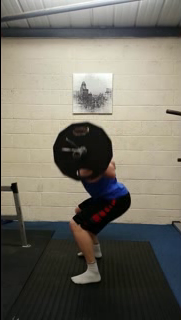
\includegraphics[height= 7cm]{algorithm/images/squat_halfway}
    }
    \subfigure[Background Subtraction Applied]{
            
\includegraphics[height= 7cm]{algorithm/images/squat_halfway_bgsub}
    }
\caption{Background Subtraction applied to a frame}
\label{fig:bgsub}
\end{figure}

Another issue with background subtraction was that moving objects in the surroundings were classified as foreground. In practice it is often difficult to find an area in the gym devoid of small levels of movement, whether it be television screens or other people in the distant background. In order to make the background subtraction more precise for fitting, it was decided to apply a final processing step. In this step, the largest object in the foreground is detected, and only this is deemed foreground. The OpenCV function \texttt{findContours} detects separate objects in an image. The volume of each detected object calculated in turn, and the one with maximum volume is considered to be the figure.

In summary, the final background subtraction algorithm utilised in the tracking phase is to perform a naive RGB subtraction to give a proposed foreground, remove shadows identified by \texttt{BackgroundSubtractorMOG2}, and return the largest remaining object as the foreground.